\documentclass[border=4pt,12pt]{standalone}
% House style for redrawn exam diagrams (diagram-v4: 0.4pt lines, filled -latex arrows, fine dashes; stipple and hatching drawn as real dots/lines (no PDF/SVG patterns, so they render in every browser and at any scale); transparent background). Every figure \input's this.
\usepackage{amsmath,amssymb}
\usepackage{txfonts}
\usepackage{pdfrender,xcolor}
% \halo{text}: label on shading. The shading stops just around each letter's outline (a thin knock-out that follows the
% glyphs, like the papers' typesetting), never a box. Owner: "I don't want a box around the text".
\newcommand{\halo}[1]{\leavevmode\rlap{\pdfrender{TextRenderingMode=2,LineWidth=2.2pt,LineJoinStyle=1,StrokeColor=white,FillColor=white}#1}#1}
\usepackage{tikz,pgfplots}
\pgfplotsset{compat=1.18}
\usetikzlibrary{arrows.meta,calc,angles,quotes,patterns,patterns.meta,intersections,positioning,decorations.markings,shapes.geometric}
% Stipple and hatching are drawn as actual dots / lines clipped to the region (path picture), NOT as pattern fills:
% SVG <pattern> fills vanish or blur when browsers scale the image, so the owner could not see the shading.
% Each dot is a 0.72pt square (keeps SVGs small; reads as a dot at print size). Dots sit on one global staggered grid, so neighbouring regions line up.
\makeatletter
\newdimen\ex@x \newdimen\ex@y \newdimen\ex@xa \newdimen\ex@ya \newdimen\ex@xb \newdimen\ex@yb \newcount\ex@row
\def\exam@stipplecolor{black!75}\def\exam@dotr{0.42pt}\def\exam@dotgap{2.5}
\def\ex@rowdots{\ifdim\ex@x<\ex@xb \pgfpathrectangle{\pgfqpoint{\dimexpr\ex@x-0.36pt\relax}{\dimexpr\ex@y-0.36pt\relax}}{\pgfqpoint{0.72pt}{0.72pt}}\advance\ex@x by \exam@dotgap pt\relax\expandafter\ex@rowdots\fi}
\def\exam@stipple{%
  \pgftransformreset% dots are sized in real points even inside scaled pictures
  \pgfpointanchor{path picture bounding box}{south west}\ex@xa=\pgf@x \ex@ya=\pgf@y
  \pgfpointanchor{path picture bounding box}{north east}\ex@xb=\pgf@x \ex@yb=\pgf@y
  \pgfsetfillcolor{\exam@stipplecolor}\pgfmathsetmacro\ex@h{\exam@dotgap/2}%
  \pgfmathtruncatemacro\ex@r{floor(\ex@ya/\ex@h)-1}\ex@row=\ex@r\relax
  \ex@y=\ex@r\dimexpr\ex@h pt\relax
  \loop\ifdim\ex@y<\ex@yb
    \pgfmathtruncatemacro\ex@c{floor(\ex@xa/\exam@dotgap)-1}\ex@x=\ex@c\dimexpr\exam@dotgap pt\relax
    \ifodd\ex@row \advance\ex@x by \ex@h pt\fi
    \ex@rowdots
    \advance\ex@y by \ex@h pt \advance\ex@row by 1
    \ifnum\numexpr\ex@row-(\ex@row/4)*4\relax=0 \pgfusepath{fill}\fi% flush every 4 rows: bounded TeX memory, few clip copies in the SVG
  \repeat\pgfusepath{fill}}
\newdimen\ex@d
\def\exam@hatch#1{% #1 = 1 for /, -1 for \ ; lines 45 degrees, 3pt apart
  \pgftransformreset
  \pgfpointanchor{path picture bounding box}{south west}\ex@xa=\pgf@x \ex@ya=\pgf@y
  \pgfpointanchor{path picture bounding box}{north east}\ex@xb=\pgf@x \ex@yb=\pgf@y
  \ex@d=\dimexpr\ex@yb-\ex@ya\relax \ex@x=\dimexpr\ex@xa-\ex@d\relax
  \loop\ifdim\ex@x<\ex@xb
    \ifnum#1>0 \pgfpathmoveto{\pgfqpoint{\ex@x}{\ex@ya}}\pgfpathlineto{\pgfqpoint{\dimexpr\ex@x+\ex@d\relax}{\ex@yb}}%
    \else \pgfpathmoveto{\pgfqpoint{\ex@x}{\ex@yb}}\pgfpathlineto{\pgfqpoint{\dimexpr\ex@x+\ex@d\relax}{\ex@ya}}\fi
    \advance\ex@x by 4.24pt
  \repeat
  \pgfsetlinewidth{0.4pt}\pgfsetstrokecolor{black}\pgfusepath{stroke}}
\def\examstipple{\exam@stipple}\def\examhatch{\exam@hatch}\def\examsetstipplecolor#1{\def\exam@stipplecolor{#1}}\def\examsetdotgap#1{\def\exam@dotgap{#1}}
\makeatother
% (legacy pattern kept for old files)
% staggered stipple like the NESA papers' dotted shading
\pgfdeclarepatternformonly{exam stipple}{\pgfpointorigin}{\pgfqpoint{2.2pt}{2.2pt}}{\pgfqpoint{2.2pt}{2.2pt}}{%
  \pgfpathcircle{\pgfqpoint{0.55pt}{0.55pt}}{0.42pt}\pgfpathcircle{\pgfqpoint{1.65pt}{1.65pt}}{0.42pt}\pgfusepath{fill}}
\tikzset{
  every picture/.style={line width=0.6pt, >={Latex[length=2mm,width=1.3mm]}},
  curve/.style={line width=0.6pt},
  open arrow/.style={-{Latex[length=2mm,width=1.3mm]}},  % owner: filled -latex heads everywhere, no open chevrons
  aux/.style={dash pattern=on 2pt off 1.5pt, line width=0.6pt},
  shade/.code={\def\exA{#1}\def\exB{none}\ifx\exA\exB\else\pgfkeysalso{fill=black!18}\fi},
  shade/.default=on,
  shade dots/.style={fill=none, path picture={\examstipple}},
  stipple color/.code={\examsetstipplecolor{#1}},
  stipple gap/.code={\examsetdotgap{#1}},
  shade dense dots/.style={fill=none, stipple gap=1.6, path picture={\examstipple}},
  shade hatch/.style={fill=none, path picture={\examhatch{1}}},
  shade hatch reverse/.style={fill=none, path picture={\examhatch{-1}}},
  shade solid/.style={fill=black},
  pt/.style={circle, fill, inner sep=1.1pt},
  open pt/.style={circle, draw, fill=white, inner sep=1.1pt},
}
\pgfplotsset{
  exam axes/.style={axis lines=middle, axis line style={->}, xlabel={$x$}, ylabel={$y$},
    xlabel style={anchor=west}, ylabel style={anchor=south}, tick label style={font=\small},
    every axis plot/.append style={line width=0.6pt, black}, samples=200, clip=false,
    enlargelimits=false, axis on top},
}

\begin{document}
% 638_q11_1: y = f(x) (no equation: traced from the crop, crop pixels y down), crossing the x-axis at a and c; the region
% between the curve and the x-axis from x=0 to x=d crosshatched as printed (house hatch both ways, rule 5).
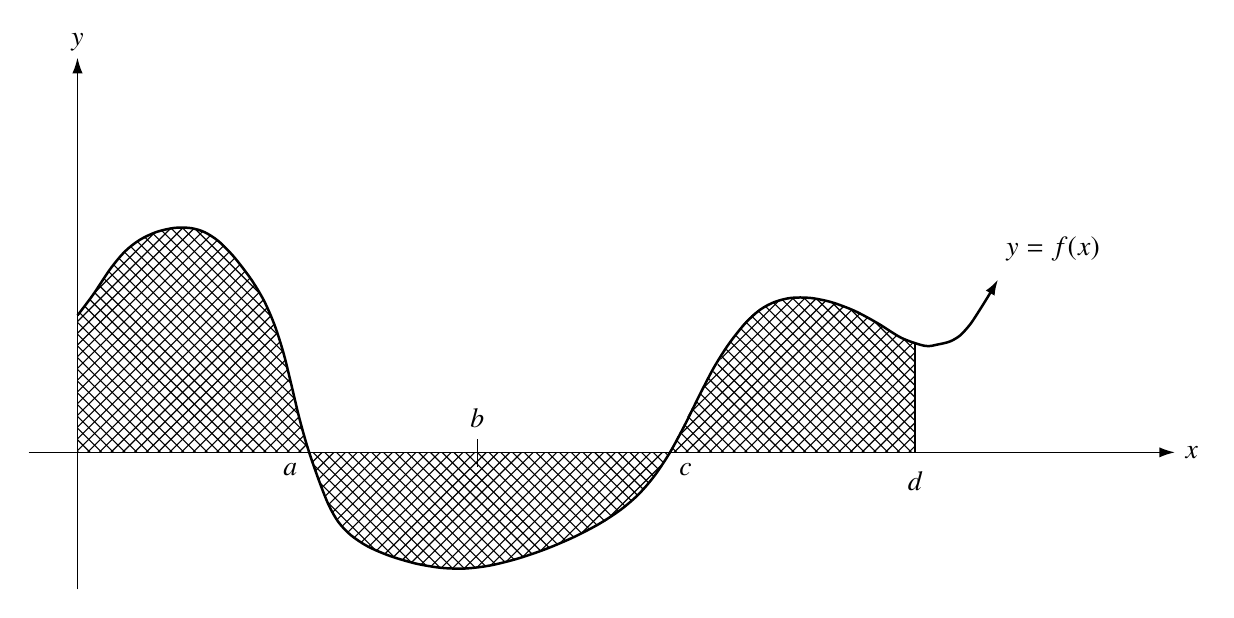
\begin{tikzpicture}[x=0.0127cm, y=-0.0127cm]
  \def\reg{(67,435) -- plot[smooth] coordinates {(67,298) (79.81,281.1) (94.27,259.4) (107.1,242.1) (119.5,229.5) (132.1,220.7) (146.6,214.4) (161.8,210.9) (176.5,210.5) (189.7,213) (201.7,218.3) (212.3,226.4) (224.1,240) (239.4,260.7) (251,278.9) (260.3,298.2) (268.3,319.5) (275.2,343.2) (281.7,369.3) (288.2,396.7) (294.9,422.4) (302.2,446.5) (310.5,469.3) (319.5,488.9) (329.5,505.2) (340.3,517.6) (352.6,527.2) (367.6,534.9) (385.8,540.9) (410.2,546.4) (432.8,550.3) (453.2,551.5) (472.5,550.1) (492.7,546) (514.4,539.1) (538,529.9) (563.4,519.1) (585.8,509.1) (602.4,499.3) (618.5,486.7) (633,472.2) (646.1,455.7) (657.7,437.2) (669.5,414.9) (681.6,390.8) (693.6,369.7) (707.2,347.5) (719.8,325.5) (730.8,309.3) (742.1,297.3) (753.4,289.4) (766.9,283.7) (782.4,280.6) (799.3,280.4) (816.9,283.1) (834.4,288.7) (852.8,297.5) (872.3,309.5) (891,321.2) (905,327)} -- (905,435) -- cycle}
  \path[shade hatch] \reg; \path[shade hatch reverse] \reg;
  \draw[->] (18,435) -- (1165,435) node[right, inner sep=3pt] {$x$};
  \draw[->] (67,572) -- (67,40) node[above, inner sep=2pt] {$y$};
  \draw[->, line width=0.9pt] plot[smooth] coordinates {(67,298) (82.52,277.4) (99.68,251.7) (114.3,234.2) (129,222.6) (146.1,214.5) (164.4,210.4) (180.7,210.7) (194.1,214.7) (208,223.7) (223.5,239.4) (240.8,262) (253.8,283.7) (264.3,308) (273.1,335.6) (280.9,367.1) (288.7,399.8) (297.1,429.8) (307.6,460.6) (318.1,487.3) (328.1,504.8) (340.3,517.7) (357.2,529) (379.2,538.5) (405.3,546.2) (430.7,550.5) (454.8,551.2) (479.6,548.2) (506.7,541.5) (534.8,532) (562.4,520.3) (588.1,507) (610.3,492.5) (628.6,476.7) (644.7,457.8) (659.8,434.9) (674.3,408.1) (689.4,377.5) (703.8,349.9) (718.7,326.4) (735,305.9) (749.8,292.4) (764.3,284.6) (780.7,280.5) (799.9,280.5) (821,284.7) (844.3,293.4) (867.8,306) (891.7,320.7) (915,328.5) (928,327) (940,324) (950,318) (960,307) (968,295) (978,279) (988,262)};
  \draw (905,327) -- (905,435);
  \draw (467,422) -- (467,450);
  \node[anchor=north east, inner sep=3pt] at (296,437) {$a$};
  \node[anchor=south, inner sep=4pt] at (467,422) {$b$};
  \node[anchor=north west, inner sep=3pt] at (660,437) {$c$};
  \node[anchor=north, inner sep=6pt] at (905,437) {$d$};
  \node[anchor=west, inner sep=2pt] at (990,232) {$y=f(x)$};
\end{tikzpicture}
\end{document}
